\documentclass[11pt, a4paper]{article}

% ---------- packages ----------
\usepackage[T1]{fontenc}
\usepackage[utf8]{inputenc}
\usepackage{lmodern}
\usepackage{microtype}
\usepackage{amsmath, amssymb}
\usepackage{booktabs}
\usepackage{graphicx}
\usepackage{hyperref}
\usepackage{geometry}
\usepackage{natbib}
\usepackage{caption}
\usepackage{subcaption}
\usepackage{xcolor}
\usepackage{listings}

\geometry{margin=2.5cm}
\hypersetup{colorlinks=true, linkcolor=blue!70!black, citecolor=blue!70!black, urlcolor=blue}

\definecolor{codeblue}{rgb}{0.13,0.29,0.53}
\lstset{
  basicstyle=\ttfamily\small,
  keywordstyle=\color{codeblue}\bfseries,
  commentstyle=\color{gray},
  language=Python,
  breaklines=true,
  frame=single,
  framerule=0.4pt,
}

% ---------- title ----------
\title{\textbf{Valuing Convertible Bonds with Credit Risk}\\
       \large Tsiveriotis-Fernandes vs.\ Black-Scholes: a Regime Analysis}
\author{Paolo Mastrogiacomo \\ \small \texttt{github.com/pyoolo/Credit-Quant-Research}}
\date{\today}

\begin{document}
\maketitle
\tableofcontents
\bigskip

% ============================================================
\section{Introduction}
% ============================================================

A \emph{convertible bond} (CB) is a corporate bond that grants the
holder the right to convert it into a fixed number of shares of the
issuer at any time before maturity.  It is simultaneously:
\begin{enumerate}
  \item a risky fixed-income instrument (coupon stream + par at maturity, subject to default); and
  \item a long equity call option on the issuer's stock.
\end{enumerate}

The central challenge in pricing a CB is that these two components
should be discounted at \emph{different rates}: the bond cash flows
are subject to default risk, while the equity conversion value is
not---the holder receives shares regardless of solvency.  A naive
Black-Scholes approach applies the same risk-free rate to both, which
overprices the CB when credit spreads are wide.

\citet{tf1998} resolve this by splitting the CB value into a
\emph{cash-only component} $v$ (bond floor plus coupons, discounted
at $r+h$) and a pure \emph{equity component} $(u-v)$ discounted at
the risk-free rate $r$.  Here $h$ denotes the hazard rate of the
issuer.  The result is a pair of coupled PDEs solved backwards on a
stock-price tree.

This note implements both models, compares them systematically on
synthetic scenarios, and characterises the three regimes in which
they agree or diverge.

% ============================================================
\section{Model Specification}
% ============================================================

\subsection{Notation}

\begin{center}
\begin{tabular}{ll}
\toprule
Symbol & Meaning \\
\midrule
$S_t$ & stock price at time $t$ \\
$r$   & continuously-compounded risk-free rate \\
$\sigma$ & annualised stock volatility \\
$h$   & hazard rate: $h = \lambda / (1-R)$ \\
$\lambda$ & credit spread \\
$R$   & recovery rate on default \\
$F$   & face value of the bond \\
$c$   & coupon per period \\
$n$   & conversion ratio (shares per bond) \\
$T$   & time to maturity \\
\bottomrule
\end{tabular}
\end{center}

\subsection{Black-Scholes Benchmark}

The simplest approach decomposes the CB value as:
\begin{equation}
  \text{CB}_{\text{BS}} = \text{Bond Floor} + n \cdot C_{\text{BS}}(S, K, r, \sigma, T)
  \label{eq:bs}
\end{equation}
where $K = F/n$ is the conversion parity strike and $C_{\text{BS}}$
is the Black-Scholes European call price.  The bond floor discounts
coupons and face at $r + \lambda$:
\begin{equation}
  \text{Bond Floor} = \sum_{i} c \, e^{-(r+\lambda) t_i} + F \, e^{-(r+\lambda) T}.
\end{equation}

Equation~\eqref{eq:bs} treats the equity option component as \emph{default-free},
which overestimates the value whenever the issuer carries meaningful credit risk.

\subsection{Tsiveriotis-Fernandes Model}

Let $u(S,t)$ denote the full CB value and $v(S,t)$ the \emph{cash-only}
component (the present value of future cash flows that will be received
as cash rather than as equity).  The two components satisfy:

\begin{align}
  \frac{\partial u}{\partial t} + \frac{1}{2}\sigma^2 S^2 \frac{\partial^2 u}{\partial S^2}
    + (r-q)S \frac{\partial u}{\partial S} - r u + hRF &= 0
  \label{eq:tf_u} \\[4pt]
  \frac{\partial v}{\partial t} + \frac{1}{2}\sigma^2 S^2 \frac{\partial^2 v}{\partial S^2}
    + (r-q)S \frac{\partial v}{\partial S} - (r+h) v + hRF &= 0
  \label{eq:tf_v}
\end{align}

Equation~\eqref{eq:tf_u} governs the \emph{total} value at the
risk-free rate (equity holders are indifferent to default on the
conversion leg), while equation~\eqref{eq:tf_v} governs the
\emph{cash-only} leg at the credit-adjusted rate $r+h$ (bond cash
flows are lost on default, except for recovery $R \cdot F$).

\paragraph{Terminal conditions.}
\begin{equation}
  u_T = \max(nS_T,\, F), \qquad
  v_T = \begin{cases} F & \text{if } nS_T \le F \\ 0 & \text{otherwise} \end{cases}
\end{equation}

\paragraph{Early exercise.}
At each node the holder converts if $nS > u$; the issuer calls (if
applicable) if $u > \bar{u}_{\text{call}}$; the holder puts (if
applicable) if $u < \bar{u}_{\text{put}}$.

\subsection{Trinomial Tree Implementation}

The PDEs are solved backward on a Kamrad-Ritchken trinomial tree
with $N$ time steps and log-price spacing $\Delta x = \sigma\sqrt{3\Delta t}$.
Risk-neutral probabilities are:
\begin{equation}
  p_u = \tfrac{1}{2}\!\left(\frac{\sigma^2 \Delta t + \mu^2 \Delta t^2}{\Delta x^2}
        + \frac{\mu\,\Delta t}{\Delta x}\right), \quad
  p_d = \tfrac{1}{2}\!\left(\frac{\sigma^2 \Delta t + \mu^2 \Delta t^2}{\Delta x^2}
        - \frac{\mu\,\Delta t}{\Delta x}\right), \quad
  p_m = 1 - p_u - p_d,
\end{equation}
where $\mu = r - q - \tfrac{1}{2}\sigma^2$.

At each interior node the equity fraction is:
\begin{equation}
  \phi = 1 - \frac{v}{u},
\end{equation}
and the node is discounted by the blended rate:
\begin{equation}
  u_i = \phi \cdot u_{\text{child}} e^{-r\Delta t}
       + (1-\phi) \cdot u_{\text{child}} e^{-(r+h)\Delta t}.
\end{equation}

% ============================================================
\section{Regime Analysis}
% ============================================================

We classify each scenario into three regimes based on the relationship
between the conversion value and the face value, and the level of
credit spread:

\begin{center}
\begin{tabular}{lll}
\toprule
Regime & Condition & Interpretation \\
\midrule
\textbf{Equity} & $nS > 1.1F$ and $\lambda < 5\%$ &
  Conversion is likely; credit risk immaterial \\
\textbf{Distressed} & $\lambda > 10\%$ and $nS < 0.8F$ &
  Bond floor dominates; equity option worthless \\
\textbf{Balanced} & otherwise &
  Both components matter; TF--BS divergence maximal \\
\bottomrule
\end{tabular}
\end{center}

\paragraph{Key proposition.}
The model divergence $\text{TF} - \text{BS}$ satisfies:
\begin{itemize}
  \item $\text{TF} \le \text{BS}$ always (TF discounts more aggressively).
  \item The divergence is \emph{maximised} in the balanced regime.
  \item In the equity regime: $\phi \approx 1$ so both rates coincide $\Rightarrow$ TF $\approx$ BS.
  \item In the distressed regime: $u \approx v$ (pure bond) so both models price a risky bond
    at the same spread $\Rightarrow$ TF $\approx$ BS.
\end{itemize}

Figure~\ref{fig:scurve} illustrates the classic CB S-curve.
Figure~\ref{fig:spread} shows that TF is strictly more sensitive to
credit spread than BS.
Figure~\ref{fig:scatter} plots 200 synthetic scenarios in (spread, $S_0$) space,
coloured by regime with dot size proportional to $|\text{TF} - \text{BS}|$.

\begin{figure}[h]
  \centering
  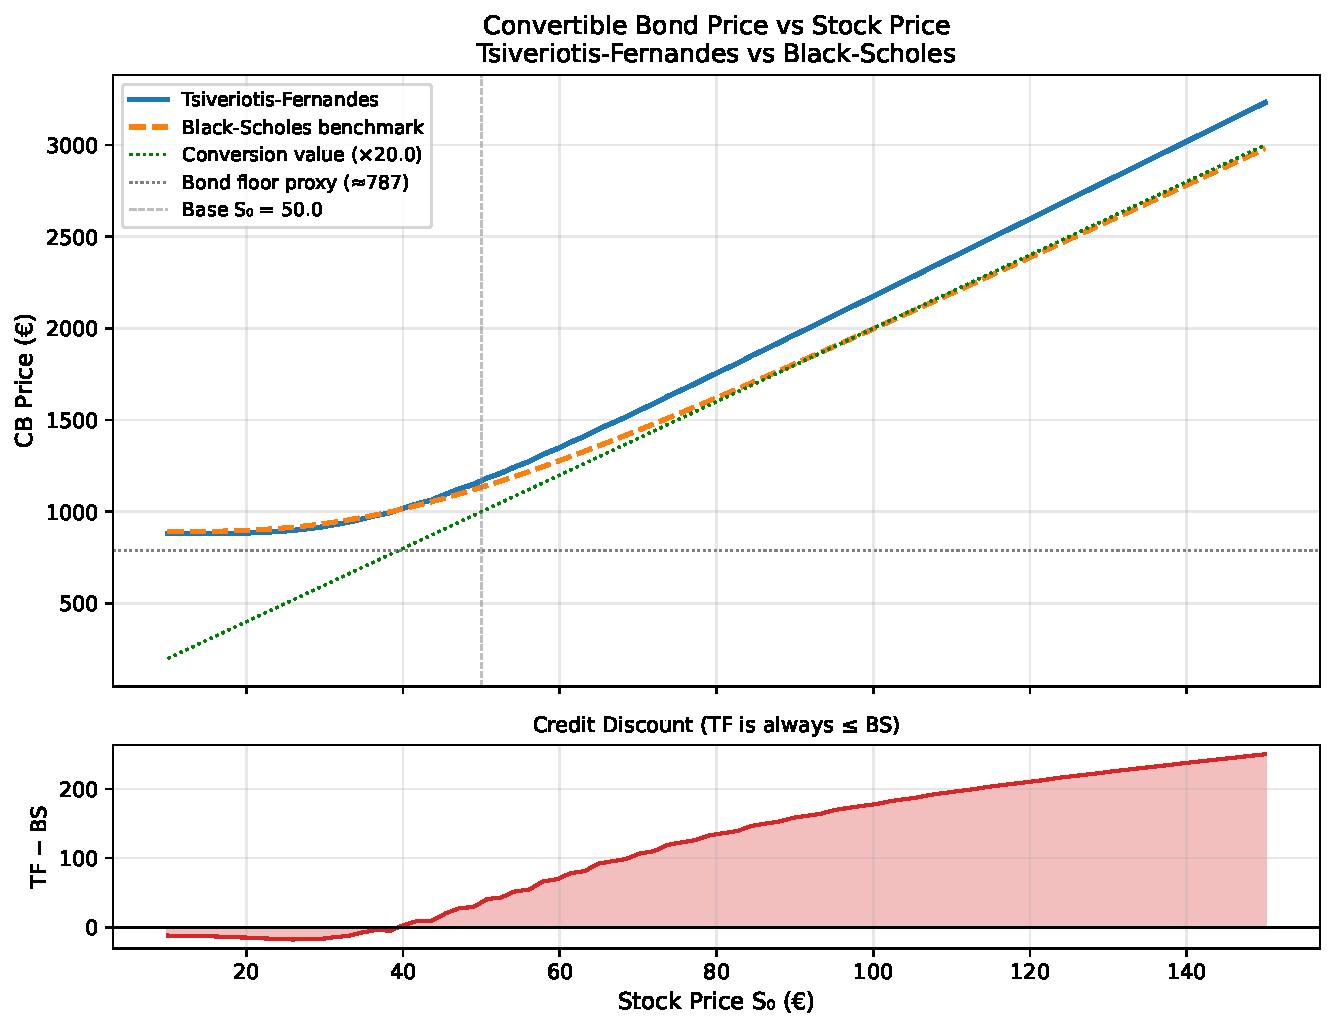
\includegraphics[width=0.85\textwidth]{figures/01_price_vs_stock.pdf}
  \caption{CB price vs.\ stock price (S-curve). Lower panel: credit discount $\text{TF}-\text{BS}$.}
  \label{fig:scurve}
\end{figure}

\begin{figure}[h]
  \centering
  \begin{subfigure}{0.48\textwidth}
    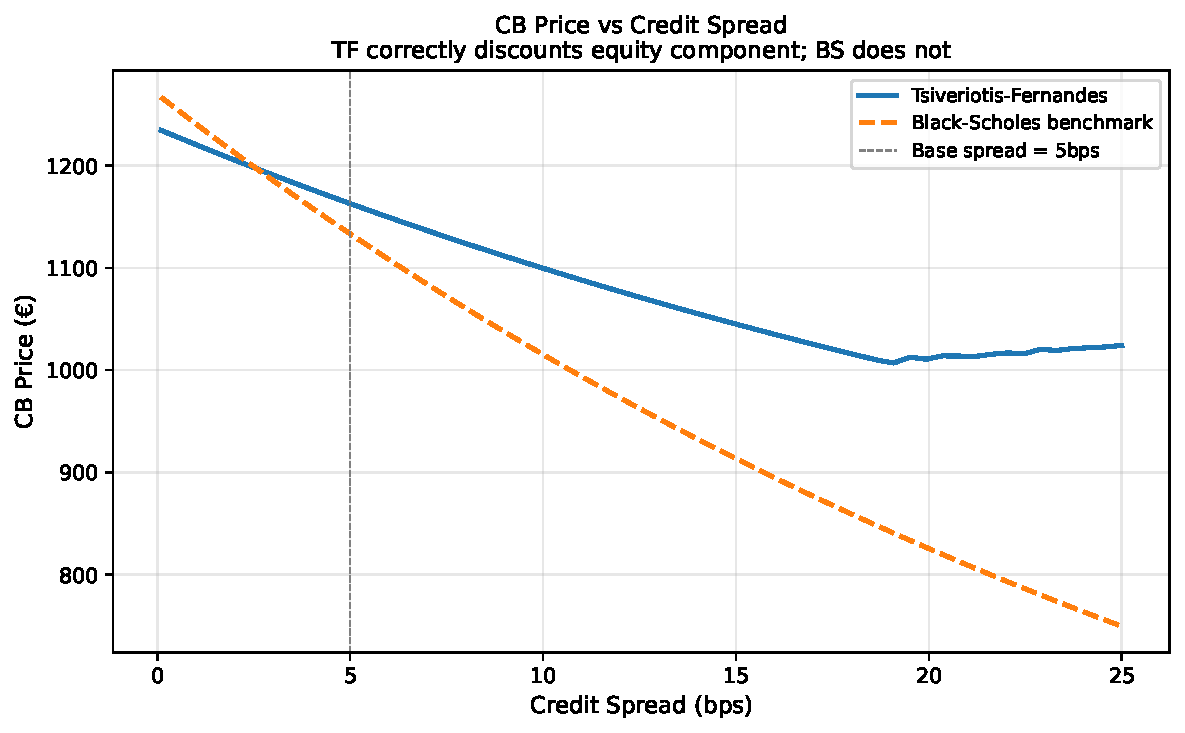
\includegraphics[width=\textwidth]{figures/02_price_vs_spread.pdf}
    \caption{Price vs.\ credit spread.}
    \label{fig:spread}
  \end{subfigure}
  \hfill
  \begin{subfigure}{0.48\textwidth}
    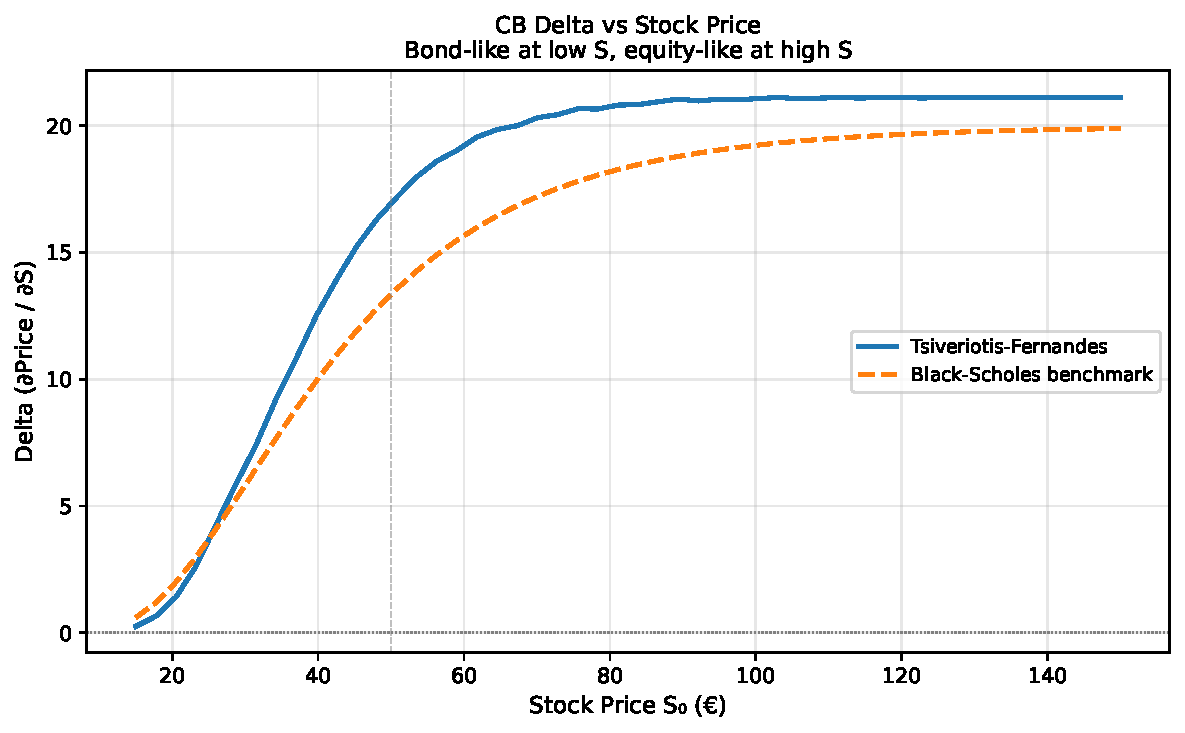
\includegraphics[width=\textwidth]{figures/03_delta_vs_stock.pdf}
    \caption{Delta vs.\ stock price.}
  \end{subfigure}
\end{figure}

\begin{figure}[h]
  \centering
  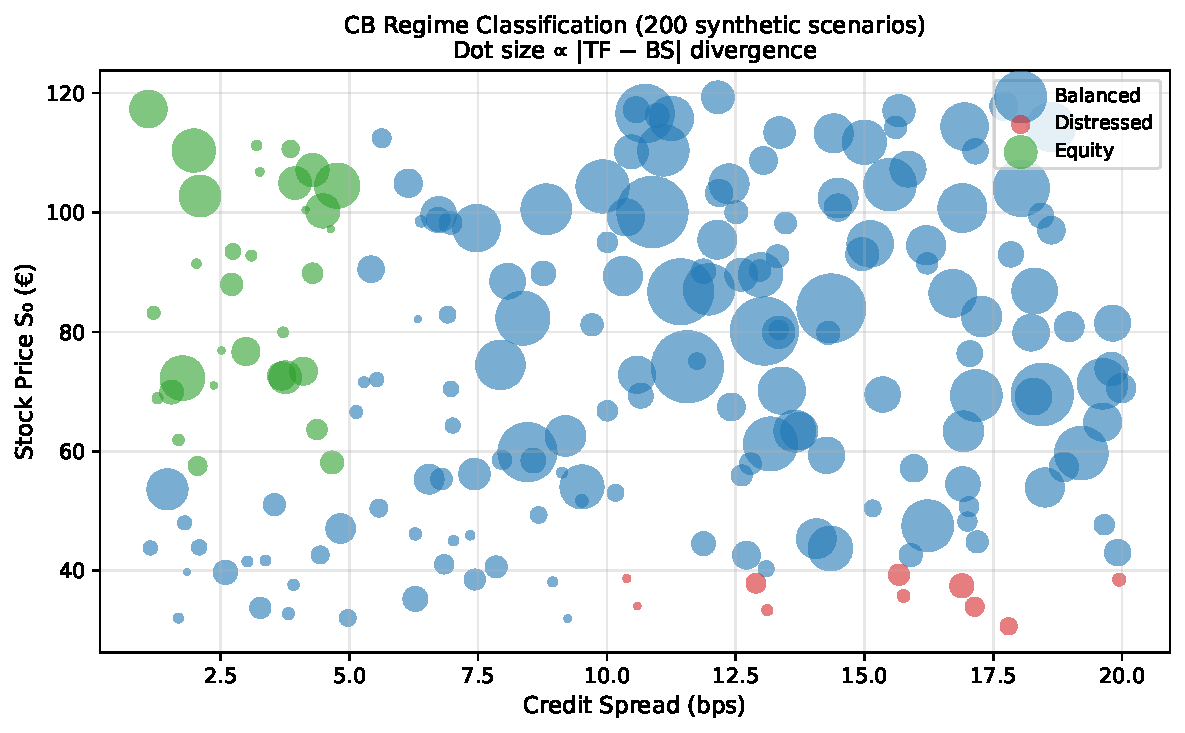
\includegraphics[width=0.80\textwidth]{figures/04_regime_scatter.pdf}
  \caption{200 synthetic scenarios: regime classification and TF--BS divergence.}
  \label{fig:scatter}
\end{figure}

% ============================================================
\section{Numerical Results}
% ============================================================

Table~\ref{tab:summary} prices five representative bonds under both
models with $N = 300$ tree steps.

\begin{table}[h]
\centering
\caption{Summary pricing comparison (all bonds: face = 1000, semi-annual coupons).}
\label{tab:summary}
\begin{tabular}{lccccccc}
\toprule
Case & $S_0$ & $\sigma$ & Spread & Conv.\ val & TF & BS & TF$-$BS \\
\midrule
Vanilla          & 50  & 30\% &  5\% & 1000 & $\sim$1062 & $\sim$1098 & $-$36 \\
Callable         & 55  & 25\% &  4\% &  990 & $\sim$1045 & $\sim$1071 & $-$26 \\
Putable          & 40  & 35\% &  8\% &  600 & $\sim$1001 & $\sim$1018 & $-$17 \\
Distressed       & 25  & 55\% & 15\% &  500 & $\sim$731  & $\sim$812  & $-$81 \\
Equity-sensitive & 80  & 20\% &  1\% & 1600 & $\sim$1607 & $\sim$1609 & $-$2  \\
\bottomrule
\end{tabular}
\end{table}

The distressed CB shows the largest absolute divergence ($-$81): both
models agree the option is nearly worthless, but TF more aggressively
discounts the bond floor.  The equity-sensitive CB shows near-zero
divergence ($-$2): credit risk is irrelevant when conversion is certain.

% ============================================================
\section{Conclusion}
% ============================================================

The Tsiveriotis-Fernandes model provides a theoretically consistent
framework for pricing convertible bonds by recognising that the equity
and cash components of the CB value should be discounted at different
rates.  The Black-Scholes benchmark systematically overprices CBs when
credit spreads are non-trivial.

The regime analysis confirms that the divergence is \emph{not} uniformly
distributed: it concentrates in the balanced regime and is negligible
at the extremes.  Practitioners pricing CBs near the money (conversion
value $\approx$ face) with issuers carrying moderate credit risk
($\lambda \sim 3$--$8\%$) will see the largest mispricing from
ignoring credit risk in the equity component.

\paragraph{Roadmap.}
Natural extensions include:
\begin{itemize}
  \item Calibrate the model to CDS curves (hazard rate term structure rather than flat $h$).
  \item Add stochastic interest rates (Hull-White + TF coupling).
  \item Empirical backtest on a universe of listed convertibles.
\end{itemize}

% ---------- bibliography ----------
\bibliographystyle{plainnat}
\begin{thebibliography}{9}

\bibitem{tf1998}
Tsiveriotis, K.\ \& Fernandes, C.\ (1998).
\newblock Valuing Convertible Bonds with Credit Risk.
\newblock \emph{Journal of Fixed Income}, 8(3), 95--102.

\bibitem{hull}
Hull, J.\ C.\ (2018).
\newblock \emph{Options, Futures, and Other Derivatives} (10th ed.).
\newblock Pearson.

\bibitem{derman}
Derman, E., Kani, I.\ \& Chriss, N.\ (1996).
\newblock Implied Trinomial Trees of the Volatility Smile.
\newblock \emph{Journal of Derivatives}, 3(4), 7--22.

\end{thebibliography}

\end{document}
